\documentclass[declaration,shortabstract, inz]{iithesis}

\usepackage[utf8]{inputenc}

\polishtitle    {Warianty gry w życie Conwaya}
\englishtitle   {Conway's Game of Life variants}
\polishabstract {Przedstawiona praca opisuje implementację projektu, umożliwiającego tworzenie i wizualizację wariantów gry w życie Conwaya opartych na planszy zbudowanej na podstawie diagramów Woronoja. Części składowe projektu to generator diagramów Woronoja oparty na algorytmie S. Fortune'a, wizualizacja gry przy zastosowaniu API OpenGl oraz ewaluator języka opisu gry.}
\englishabstract{This paper describes the project, which alowes, creation and visualization of Conway's Game of Life variants, on a a board made of Voronoi diagrams. Project consist of Voronoi diagrams generator using S. Fortune's algoritm, game visualisation using OpenGl API and game description language evaluator.}
\author         {Marcin Rogala}
\advisor        {dr hab. Jan Otop}
\date          {25 grudnia 2020}
\transcriptnum {300084}
\advisorgen    {dr hab. Jan Otopa}


\usepackage{amsmath,amsthm,natbib, caption, mathtools,amsfonts,graphicx,hyperref}
\usepackage[ruled,vlined]{algorithm2e}

\graphicspath{ {./images/} }

\theoremstyle{definition} \newtheorem{definition}{Definicja}[]
\theoremstyle{plain} \newtheorem{remark}[definition]{Obserwacja}
\theoremstyle{plain} \newtheorem{theorem}[definition]{Twierdzenie}
\theoremstyle{plain} \newtheorem{example}{Przykład}[definition]
\theoremstyle{plain} \newtheorem{lemma}[definition]{Lemat}

\begin{document}

\chapter{Wprowadzenie}
\section{Gra w życie}
Gra w życie, została zaprezentowana w 1970 roku przez Johna Conwaya.  Jest to gra bez graczy co oznacza, że jej ewolucja zależy tylko od stanu początkowego bez późniejszych ingerencji człowieka. Planszą jest dwu wymiarowa siatka kwadratowych komórek, z których każda ma 8 sąsiadów. Każda komórka może być żywa lub martwa. W standardowej grze obowiązują tylko trzy reguły:

\begin{itemize}
\item martwa komórka rodzi jeśli ma dokładnie 3 żywych sąsiadów.
\item żywa komórka umiera z zatłoczenia, jeśli ma więcej niż 3 żywych sąsiadów
\item żywa komórka umiera z samotności jeśli ma mniej niż 2 żywych sąsiadów
\end{itemize}

Przedstawione przez Conwaya proste zasady pozwoliły zachować równowagę pomiędzy rozrostem i zanikaniem struktur.

Gra w życie ma wiele ciekawych właściwości. Jedną z nich jest równoważność maszynie Turinga, co oznacza, że ma takie same możliwości obliczeniowe jak komputer z nieskończoną pamięcią i brakiem ograniczeń czasowych. Przy użyciu gry~w~życie możliwa jest konstrukcja bramek logicznych oraz implementacja różnych systemów komputerowych. Gra może przebiegać chaotycznie lub według jednego z ustalonych wzorców: 
\begin{itemize}
	\item stabilny -- pozostają niezmienne bez względu na kolejne przekształcenia
	\item oscylatory -- zmieniają się cyklicznie, regularnie wracają do poprzednich stanów
	\item statki -- oscylatory zmieniające swoją pozycję na planszy
\end{itemize}

Gra Conwaya jest przykładem automatu komórkowego, które często wykorzystywane są do przeprowadzania symulacji komputerowych. 
Max Brenner w swoim artykule \cite{brenner} przedstawił symulację rozprzestrzeniania się wirusa COVID-19, co bardzo dobrze pokazuje możliwości, jakie dają nam modyfikacje gry w życie oraz bardziej rozbudowane automaty komórkowe.

\section{Opis projektu}

Przedstawiona praca opisuje projekt pozwalający na definiowanie zasad gry w życie używając prostego języka. Gra odbywa się na planszy będącej diagramem Woronoja, co istotnie narusza jedną z właściwości automatów komórkowych, mianowicie komórki automatu różnią się od siebie. Pozwala to wprowadzić element nieregularności oraz upodabnia grę do prawdziwego życia, w którym elementy symulacji mają istotne różnice wynikające se swojej budowy lub środowiska.
Weźmy za przykład ludzi, którzy mają różną liczbę osób w swoim otoczeniu, co wpływa na wiarygodność symulacji przeprowadzonych na standardowej siatce kwadratów.

Pierwszą częścią pracy jest przedstawienie algorytmu Fortune pozwalającego na generowanie diagramów Woronoja. Algorytm przyjmuje na wejściu zbiór punktów oraz opierając się na technice zamiatania generuje na ich podstawie diagram.
Algorytm Fortune rozpatruje względem współrzędnej $y$ następujące wydarzenia:
\begin{itemize}
	\item site event - miotła napotyka kolejny punkt z wejściowego zbioru
	\item circle event - miotła napotyka wydarzenie będące niwelacją jednej z paraboli wykorzystywanej do wyznaczania krawędzi diagramu.
\end{itemize}
Po rozpatrzeniu wszystkich wydarzeń wynikiem działania algorytmu są krawędzie oraz graf sąsiedztwa pól diagramu Woronoja.

Drugą częścią pracy jest opis gramatyki oraz mechanizmu prasowania i ewaluacji języka opisu gry. Parser tworzonych przez użytkowników programów wykorzystuje bibliotekę PEGTL, która opiera się na gramatycę PEG oraz parsowaniu z góry na dół. Wynikiem parsowania jest abstrakcyjne drzewo rozkładu języka, które jest następnie ewaluowane do odpowiednich funkcji opisujących grę w życie.

Kolejna część, to opis wykorzystania API OpenGl do przeprowadzenia wizualizacji gry.

Pracę uzupełnia opis istniejących narzędzi i algorytmów do przeprowadzania symulacji z użyciem gry w życie.

\chapter{Diagramy Woronoja}

\section{Definicja}
Niech $S$ będzie skończonym zbiorem parami różnych dwuwymiarowych punktów o współrzędnych rzeczywistych. Punkty zbioru $S$, nazywane będą centrami.

\begin{definition}
	   \textit{Polem diagramu Woronoja} odpowiadającemu punktowi $p \in S$ oznaczamy $Vor_S(p) = \{ x \quad | \quad x 		\in \mathbb{R}^2 \land \forall p' \in S \quad \space dist(x, p) \leq dist(x, p')\}$, gdzie $dist$ oznacza odległość euklidesową dwóch punktów.
\end{definition}

\begin{definition}
	   \textit{Diagram Woronoja}, to zbiór $\{ Vor_S(p) \quad  | \quad p \in S\}$.
\end{definition}

\begin{example}
Przykładowy diagram Woronoja z zaznaczonymi $10$ centrami.
	\begin{center}
		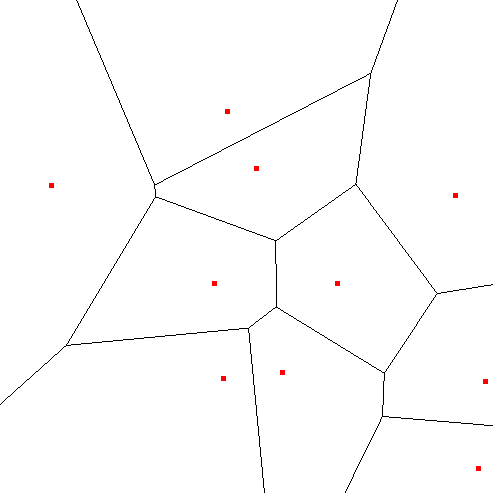
\includegraphics[width=0.7\textwidth]{ExampleDiagram}
	\end{center}
\end{example}

\section{Algorytm Fortunea}
\subsection{Opis algorytmu}
Jednym ze sposobów  generowania diagramów Woronoja jest algorytm zaproponowany przez Johna Fortunea oparty na technice zamiatania \cite{miotla}. 

\begin{definition}
\textit{Miotłą} nazywamy poziomą linię poruszającą się od dołu do góry planszy. Wszystkie punkty poniżej miotły zostały już rozpatrzone przez algorytm, natomiast punkty powyżej miotły zostaną rozpatrzone, gdy miotła dojdzie do ich wysokości.
\end{definition}

Najważniejszą strukturą algorytmu jest towarzysząca miotle linia brzegowa. Składa się ona z parabol, rozpinających się na rozpatrzonymi przez miotłę punktami oraz nieukończonych krawędzi diagramu. W czasie trwania algorytmu parabole rozszerzają się, a ich przecięcia wyznaczają krawędzie. Parabola, która tworzy pole z centrum $p = (x_p, y_p)$ jest zbiorem $\{ x \quad | \quad x \in \mathbb{R}^2 \land dist(p, x) = dist(p_s, x) \}$, gdzie przez $p_s$ oznaczamy punkt na miotle znajdujący się najbliżej $x$. 

\begin{remark}
Punkt przecięcia sąsiednich parabol jest równo odległy od centrów, które definiują te parabole.
\end{remark}

Wyznaczymy wzór $f(x)$ parabol znajdujących się w linii brzegowej.
Niech $y_s$ oznacza wysokość, na której znajduje się miotła, a $(x_c, y_c)$ będzie centrum pola, które tworzy parabola. 

\begin{align*}
	dist((x_c, y_c), (x, f(x))) &= dist((x, y_s) (x, f(x))) \\
	\sqrt{(x_c - x)^2 + (y_c - f(x))^2} &= \sqrt{(x - x)^2 + (y_s - f(x))^2} \\
	(x_c - x)^2 + (y_c - f(x))^2 &= (y_s - f(x))^2 \\
	(x_c - x)^2 &= (y_s - f(x))^2 - (y_c - f(x))^2 \\ 
	(x_c - x)^2 &= 2f(x)y_c - 2f(x)y_s + y_s^2 - y_c^2 \\
	(x_c - x)^2 + (y_c^2 - y_s^2) &= 2f(x)(y_c - y_s) \\
	f(x) &= \frac{(x - x_c)^2}{2(y_c - y_s)} + \frac{y_c^2 - y_s^2}{2(y_c - y_s)} \\
	f(x) &= \frac{(x - x_c)^2}{2(y_c - y_s)} + \frac{y_c + y_s}{2}
\end{align*}

Korzystając z otrzymanego wzoru, możemy w łatwy sposób wyliczać między innymi przecięcia parabol z innymi obiektami w linii brzegowej.

Poruszająca się przez planszę miotła napotyka dwa rodzaje wydarzeń.

\begin{itemize}
	\item site event -- dotarcie do nowego puntu ze zbioru $S$
	\item circle event -- zniwelowanie jednej z parabol w linii brzegowej
\end{itemize}

\subsubsection{Site event -- obsługa}
\label{sec:site}
Napotykając nowe centrum, musimy dodać do linii brzegowej nową parabolę, dzieląc jedną z istniejących na dwie części. W tym celu przeszukujemy linię brzegową poszukując paraboli leżącej bezpośrednio pod nowym centrum. To przeszukiwanie będzie miało kluczowy wpływ na złożoność algorytmu. 

\begin{example}
	Zmienione elementy linii brzegowej po obsłużeniu nowego centrum.
	
	\begin{center}
		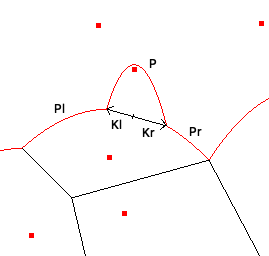
\includegraphics[width=0.6\textwidth]{ExampleSiteEvent}
	\end{center}
\end{example}

Odnaleziona parabola zostaję zastąpiona ciągiem elementów:
\begin{align}
 	Pl, Kl, P, Kr, Pr
\end{align}
Gdzie $Pl, Pr$ to kopie rozdzielanej paraboli. $P$ to nowa parabola utworzona przez dodawane centrum. $Kl, Kr$ to nowe krawędzie rozszerzające się w przeciwnych kierunkach. Punktem startowym dodawanych krawędzi jest punkt na rozdzielanej paraboli znajdujący się pod nowym centrum.

Pozostaje sprawdzić, czy parabole, które dodaliśmy do linii brzegowej zostaną kiedyś zniwelowane i czy konieczne jest dodanie odpowiednich wydarzeń. 
Parabola zostanie zniwelowana przez swoich sąsiadów jeśli zachodzą dwa warunki:
\begin{itemize}
	\item parabola nie jest skrajnie lewym lub skrajnie prawym elementem linii brzegowej
	\item krawędzie (półproste) będące sąsiadami paraboli, przecinają się
\end{itemize}
Aby dodać nowe wydarzenie polegające na ściśnięciu paraboli przez jej sąsiadów, musimy poznać jego współrzędną $y$. 
Weźmy ciąg elementów linii brzegowej:
\begin{align}
	P1, K1, P2, K2, P3
\end{align}
Punkt $p_i = (x_i, y_i)$ będący punktem przecięcia krawędzi $K1$ i $K2$ jest też miejscem przecięcia parabol $P1$ i $P3$, co czyni $y_i$
wysokością na której $P2$ zostanie ściśnięte przez $P1$ i $P3$. W tym momencie $p_i$ będzie równo odległe od centrów parabol $P1, P2, P3$. Centra te będą leżały na okręgu o środku $p_i$, skąd wzięła się nazwa wydarzenia.


\subsubsection{Circle event -- obsługa}
\label{sec:circle}
Rozpatrzmy następujący ciąg elementów w linii brzegowej:
\begin{align}
	P1, K1, P2, K2, P3
\end{align}
Załóżmy, że parabola $P2$ zostaje ściśnięta i musimy usunąć ją z linii brzegowej. Leżące po jej bokach krawędzie $K1, K2$ nie będą już rosły. Powinny zostać usunięte i oznaczone jako gotowe krawędzie diagramu. Pozostaje dodać nową krawędź pomiędzy parabolami $P1$ i $P3$ oraz podobnie jak podczas obsługi nowego centrum sprawdzić, czy konieczne jest dodanie wydarzeń niwelacji $P1$ i $P3$.


 \begin{example}
	Obsłużone wydarzenie, usunięto parabolę $P2$ oraz krawędzie $K1$~i~$K2$. W ich miejsce dodana została krawędź $K3$.
	
	\begin{center}
		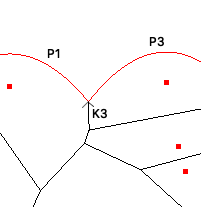
\includegraphics[width=0.6\textwidth]{ExampleCircleEvent}
	\end{center}
\end{example}

\newpage

\subsection{Implementacja}

\subsubsection{Pseudokod}
Poniższy pseudokod pokazuje, bardzo uproszczony sposób rozpatrywania wydarzeń. Wydarzenia trzymane są na stosie, zaimplementowanym przy użyciu $priority\_queue$ ze standardowej biblioteki języka $C++$.

\begin{algorithm}[H]
\SetAlgoLined
	Kolejka wydarzeń eventQueue zawiera wszystkie wydarzenia typu site event.\\
 \While{eventQueue nie jest pusta}{
 	currentEvent = eventQueue.top(); \\
  \eIf{currentEvent jest typu site event}{
   		handleSiteEvent(currentEvent);
   }{
   		handleCircleEvent(currentEvent);
  }
 }
 \caption{Pseudokod algorytmu}
\end{algorithm}

\subsubsection{Linia brzegowa}
Linia brzegowa -- \textit{Beachline}, jest najważniejszą strukturą całego algorytmu. Zawiera ona listę struktur \textit{BeachlineField}, przechowującą elementy znajdujące się w linii brzegowej. Wszystkie funkcje, których złożoność nie została określona, działają ze stałą złożonością. Najważniejsze funkcje \textit{Beachline} to:

\begin{itemize}
\item \textit{findParabolaForNewSite} -- wyszukująca parabolę z linii brzegowej, która znajduje się bezpośrednio pod nowym centrum. Funkcja oblicza przecięcia parabol, z ich sąsiadami co pozwala poznać przedział na jakim się one znajdują. Złożoność tej funkcji to $O(n)$, gdzie $n$ to rozmiar linii brzegowej.

\item \textit{handleSiteEvent} -- wykonująca niezbędne operacje opisane w \hyperref[sec:site]{Site event -- obsługa}. Złożoność tej funkcji to $O(n)$, gdzie $n$ to rozmiar linii brzegowej.

\item \textit{handleCircleEvent} -- wykonująca niezbędne operacje opisane w \hyperref[sec:circle]{Circle event -- obsługa}.

\item \textit{addCircleEvents} -- funkcja dodająca niezbędne wydarzenia typu \textit{circle event}, dla nowych elementów linii brzegowej.
\end{itemize}

\textit{Beachline} zawiera dużo funkcji pomocniczych, pomagających obsługiwać wydarzenia oraz wykonywać niezbędne obliczenia na parabolach i krawędziach. Niektóre z tych funkcji to:

\begin{itemize}
\item \textit{addNewField} -- funkcja dodająca nowy element do linii brzegowej.
\item \textit{removeField} -- funkcja usuwająca element z linii brzegowej.
\item \textit{parabolaHalfEdgeIntersection} -- funkcja wyznaczająca punkt przecięcia paraboli z półprostą.
\item \textit{edgesIntersection} -- funkcja wyznaczająca przecięcie półprostych.
\item \textit{completePolygons} -- funkcja czyszcząca linię brzegową po zakończonej pracy oraz oznaczająca ostatnie krawędzie jako zakończone. Złożoność tej funkcji to $O(n)$, gdzie $n$ to rozmiar linii brzegowej.
\end{itemize}

\textit{Beachline} przechowuje także wynikowe krawędzie algorytmu oraz uzyskany graf połączeń pól diagramu.

\subsubsection{Pozostałe struktury}
\begin{itemize}
	\item \textit{Event} -- przechowuje informacje dotyczące wydarzeń przechowywanych w~\textit{eventQueue}.
	\item \textit{Parabola} -- reprezentuje parabolę przechowywaną w linii brzegowej.
	\item \textit{HalfEdge} -- reprezentuję nieukończoną krawędź (półprostą), która rozszerza się w trakcie trwania algorytmu.
	\item \textit{Edge} -- reprezentuje ukończona krawędź.
\end{itemize}

\section{Inne algorytmy}

\chapter{Język opisu gry}
\section{Główne programy}
\section{Konstrukcje językowe}

\chapter{Parser}

\chapter{Przykłady użycia}
\chapter{Inne narzędzia}
\section{Golly}
\subsection{Opis}
\subsection{Algorytm}
\section{PlayGameOfLife}

%\nocite{}
\bibliographystyle{plain}
\bibliography{bibliography}

\end{document}
